\documentclass{beamer}
\input{../utils/preamble}
\createdgmtitle{10}

%--------------------------------------------------------------------------------
\begin{document}
%--------------------------------------------------------------------------------
\begin{frame}[noframenumbering,plain]
\titlepage
	\resetonslide	
\end{frame}
%=======
\begin{frame}{Recap of Previous Lecture}
	\myfootnotewithlink{https://arxiv.org/abs/1806.07366}{Chen R. T. Q. et al. Neural Ordinary Differential Equations, 2018}   
	\begin{block}{Continuous-Time Dynamics (Neural ODE)}
		\vspace{-0.5cm}
		\begin{align*}
			\frac{d \bx(t)}{dt} &= \bv_{\btheta}(\bx(t), t);\quad \text{where } \bx(t_0) = \bx_0. \\
			\bpsi_t(\bx_0) &= \int^{t_1}_{t_0} \bv_{\btheta}(\bx(t), t) d t  + \bx_0 \approx {\color{teal}\ODESolve_v(\bx_0, \btheta, t_0, t_1)}.
		\end{align*}
		\vspace{-0.5cm}
	\end{block}
	\begin{itemize}
		\item $\bv_{\btheta}: \bbR^m \times [t_0, t_1] \rightarrow \bbR^m$ is a vector field.
		\item $\bpsi: \bbR^m \times [t_0, t_1] \rightarrow \bbR^m$ is a flow (the solution of ODE):
	\end{itemize}
	\begin{block}{Euler Update Step (ODESolve)}
		\vspace{-0.3cm}
		\[
  			\bx(t + h) = \bx(t) + h \cdot \bv_{\btheta}(\bx(t), t)
		\]
	\end{block}
	More advanced numerical methods (such as Runge-Kutta) are often used instead of unstable Euler update step.
\end{frame}
%=======
\begin{frame}{Recap of Previous Lecture}
	\myfootnotewithlink{https://arxiv.org/abs/1810.01367}{Grathwohl W. et al. FFJORD: Free-form Continuous Dynamics for Scalable Reversible Generative Models, 2018}  
	\vspace{-0.3cm}
	\[
 		\frac{d \bx(t)}{dt} = \bv_{\btheta}(\bx(t), t);\quad \bx(t_0) = \bx_0
	\]
	\vspace{-0.3cm}
	\begin{itemize}
		\item Suppose $\bx(0)$ is a random variable with density~$p_0(\bx)$. Then, $\bx(t)$ is a random variable with density~$p_t(\bx)$.
		\item $p_t(\bx) = p(\bx, t)$ describes the \textbf{probability path} between $p_0(\bx)$ and $p_1(\bx)$.
	\end{itemize}
	\vspace{-0.3cm}
	\begin{figure}
		\centering
		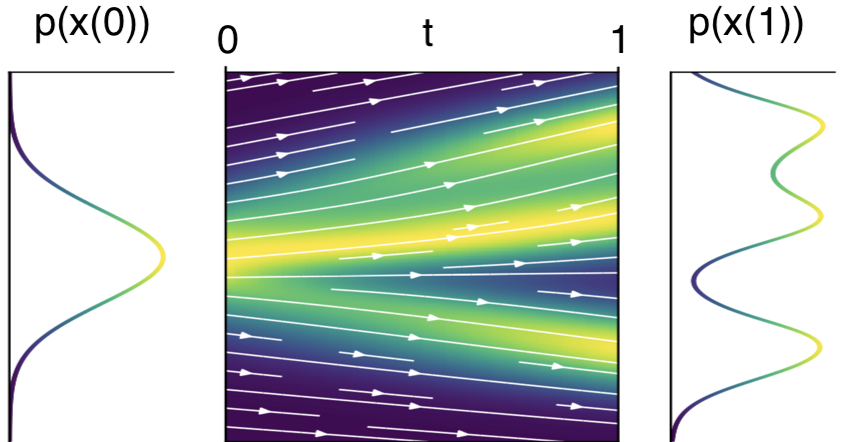
\includegraphics[width=0.7\linewidth]{figs/cnf_flow.png}
	\end{figure}
\end{frame}
%=======
\begin{frame}{Recap of Previous Lecture}
	\myfootnotewithlink{https://arxiv.org/abs/1806.07366}{Chen R. T. Q. et al. Neural Ordinary Differential Equations, 2018}   
	\begin{block}{Theorem (Picard)}
		If $\bv$ is uniformly Lipschitz continuous in $\bx$ and continuous in $t$, then the ODE has a \textbf{unique} solution.
	\end{block}
	This means the ODE can be \textbf{uniquely inverted}:
	\begin{align*}
		\bx(1) &= \bx(0) + \int_{0}^{1} \bv_{\btheta}(\bx(t), t) dt \\
		\bx(0) &= \bx(1) + \int_{1}^{0} \bv_{\btheta}(\bx(t), t) dt
	\end{align*}
	\textbf{Note:} Unlike discrete-time NF, $\bv$ need not be invertible (uniqueness ensures bijectivity).
	
	How can we compute $p_t(\bx)$ for any $t$?
\end{frame}
%=======
\begin{frame}{Outline}
	\tableofcontents
\end{frame}
%=======
\section{Probability Flow ODE}
%=======
\begin{frame}{Probability Flow ODE}
	\myfootnotewithlink{https://arxiv.org/abs/2011.13456}{Song Y., et al. Score-Based Generative Modeling through Stochastic Differential Equations, 2020}
	\begin{block}{ODE and Continuity Equation}
		\vspace{-0.3cm}
		\[
			d\bx = \bv(\bx, t) dt
		\]
		\[
			\frac{d \log p_t(\bx(t))}{d t} = - \tr \left( \frac{\partial \bv(\bx, t)}{\partial \bx} \right) 
			\quad  \Leftrightarrow  \quad 
 			\frac{\partial p_t(\bx)}{\partial t} = - \diver(\bv(\bx, t) p_t(\bx))
 		\]
		The only source of randomness is the initial distribution $p_0(\bx)$.
	\end{block}
	\eqpause
	\begin{block}{SDE and KFP Equation}
		\vspace{-0.3cm}
		\[
			d\bx = \bff(\bx, t) dt + g(t) d \bw
		\]
 		\[
 			\frac{\partial p_t(\bx)}{\partial t} = - \diver(\bff(\bx, t) p_t(\bx)) + \frac{1}{2}g^2(t) \Delta_{\bx}p_t(\bx)
 		\]
		Now there are two sources of randomness: the initial distribution $p_0(\bx)$ and the Wiener process $\bw(t)$.
	\end{block}
\end{frame}
%=======
\begin{frame}{Probability Flow ODE}
	\myfootnotewithlink{https://arxiv.org/abs/2011.13456}{Song Y., et al. Score-Based Generative Modeling through Stochastic Differential Equations, 2020}
	\begin{block}{Theorem}
		Suppose the SDE $d\bx = \bff(\bx, t) dt + g(t) d \bw$ induces the probability path $p_t(\bx)$.
		Then, there exists an ODE with the same probability path $p_t(\bx)$, given by
		\vspace{-0.3cm}
		\[
			d\bx = \bv(\bx, t) dt = \left(\bff(\bx, t) -\frac{1}{2} g^2(t) \frac{\partial}{\partial \bx} \log p_t(\bx) \right) dt
		\]
		\vspace{-0.7cm}
	\end{block}
	\eqpause
	\begin{figure}
		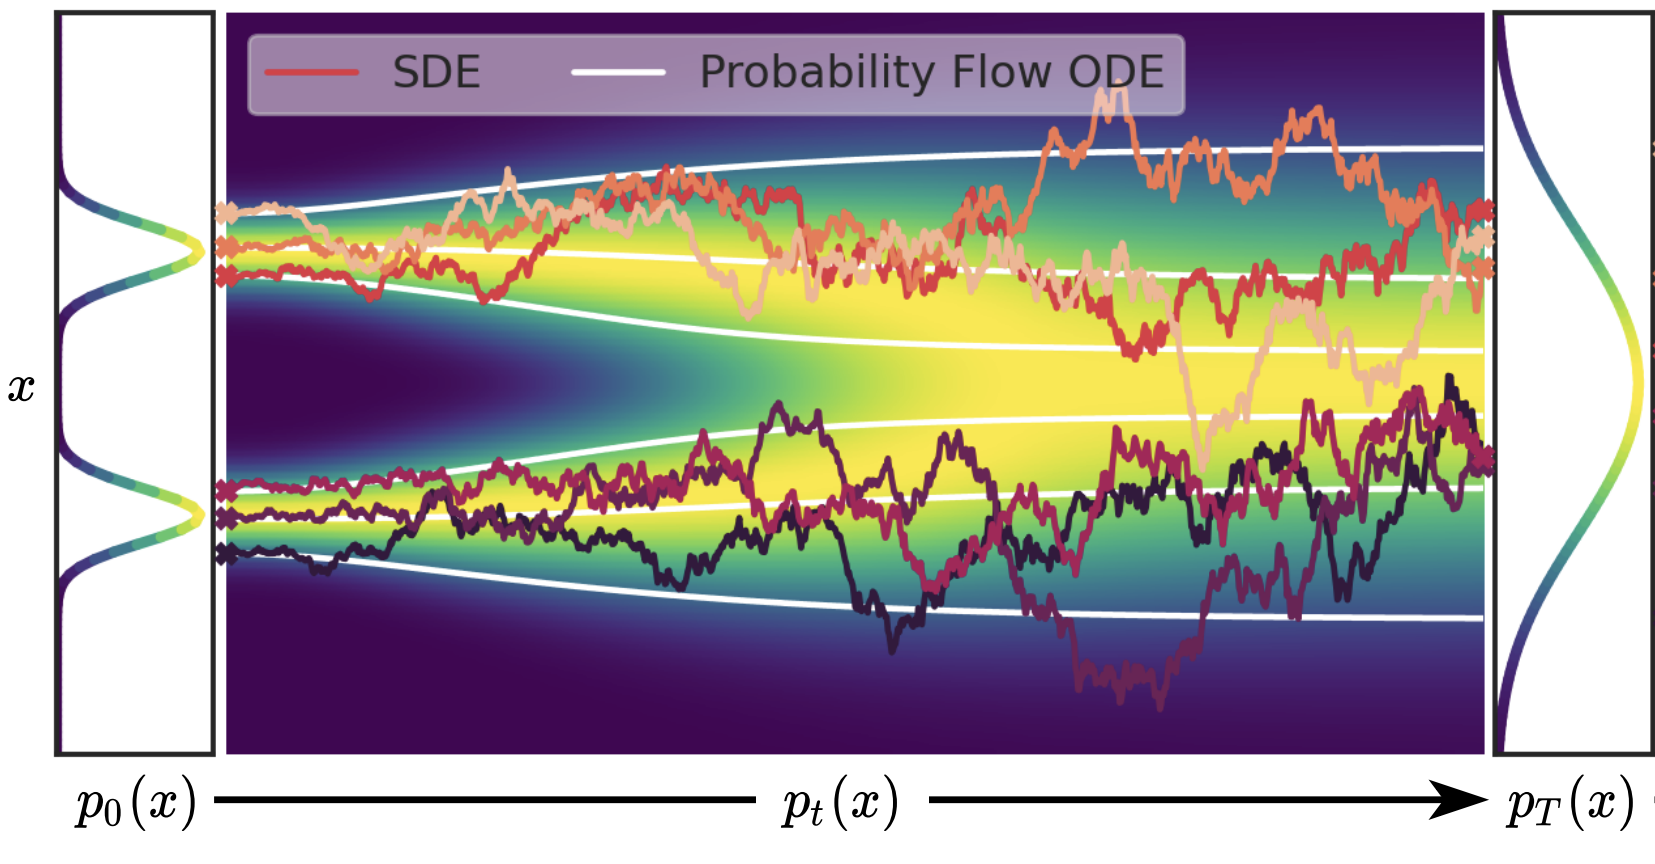
\includegraphics[width=0.75\linewidth]{figs/probability_flow}
	\end{figure}
\end{frame}
%=======
\begin{frame}{Probability Flow ODE}
	\myfootnotewithlink{https://arxiv.org/abs/2011.13456}{Song Y., et al. Score-Based Generative Modeling through Stochastic Differential Equations, 2020}
	\vspace{-0.3cm}
	\begin{block}{Theorem}
		Suppose the SDE $d\bx = \bff(\bx, t) dt + g(t) d \bw$ induces the probability path $p_t(\bx)$.
		Then, there exists an ODE with the same probability path $p_t(\bx)$, given by
		\vspace{-0.3cm}
		\[
			d\bx = \bv(\bx, t) dt = \left(\bff(\bx, t) -\frac{1}{2} g^2(t) \frac{\partial}{\partial \bx} \log p_t(\bx) \right) dt
		\]
		\vspace{-0.7cm}
	\end{block}
	\begin{block}{Proof}
 		\vspace{-0.7cm}
 		{\small
 		\begin{multline*}
 			\frac{\partial p_t(\bx)}{\partial t} = \tr\left( - \frac{\partial}{\partial \bx} \bigl[ \bff(\bx, t) p_t(\bx)\bigr] + \frac{1}{2} g^2(t) \frac{\partial^2 p_t(\bx)}{\partial \bx^2} \right) 
			\nextonslide{= \\ = \tr\left( - \frac{\partial}{\partial \bx} \left[ \bff(\bx, t) p_t(\bx) - \frac{1}{2} g^2(t) {\color{violet}\frac{\partial p_t(\bx)}{\partial \bx}} \right]  \right)}
			\nextonslide{ = \\ =  \tr\left( - \frac{\partial}{\partial \bx} \left[ \bff(\bx, t) p_t(\bx) - \frac{1}{2} g^2(t) {\color{violet}p_t(\bx) \frac{\partial}{\partial \bx} \log p_t(\bx)} \right]  \right)}
			\nextonslide{= \\ =  \tr\left( - \frac{\partial}{\partial \bx} \left[ \left( {\color{teal}\bff(\bx, t) - \frac{1}{2} g^2(t) \frac{\partial}{\partial \bx} \log p_t(\bx)}\right) p_t(\bx) \right]  \right)}
 		\end{multline*}
 		}
 	\end{block}
\end{frame}
%=======
\begin{frame}{Probability Flow ODE}
	\myfootnotewithlink{https://arxiv.org/abs/2011.13456}{Song Y., et al. Score-Based Generative Modeling through Stochastic Differential Equations, 2020}
	\begin{block}{Proof (Continued)}
 		\vspace{-0.7cm}
 		\begin{multline*}
 			\frac{\partial p_t(\bx)}{\partial t} =  \tr\left( - \frac{\partial}{\partial \bx} \left[ \left( {\color{teal}\bff(\bx, t) - \frac{1}{2} g^2(t) \frac{\partial}{\partial \bx}\log p_t(\bx)}\right) p_t(\bx) \right]  \right) 
			\nextonslide{=\\ =  \tr\left( - \frac{\partial}{\partial \bx} \left[ {\color{teal}\bv(\bx, t)} p_t(\bx) \right]  \right) = -  \diver\left(\bv(\bx, t) p_t(\bx)\right)}
 		\end{multline*}
		\eqpause
		\[
			\bv(\bx, t) = \bff(\bx, t) -\frac{1}{2} g^2(t) \frac{\partial}{\partial \bx} \log p_t(\bx); \quad \tilde{g}(t) = 0
		\]
	 	\[
	 		d \bx = \bv(\bx, t) dt + 0 \cdot d \bw = \left(\bff(\bx, t) -\frac{1}{2} g^2(t) \frac{\partial}{\partial \bx} \log p_t(\bx) \right) dt
	 	\]
		\[
			\frac{\partial p_t(\bx)}{\partial t} = - \diver(\bv(\bx, t) p_t(\bx)) + \frac{1}{2}\tilde{g}^2(t) \Delta_{\bx}p_t(\bx)
		\]
 	\end{block}
\end{frame}
%=======
\begin{frame}{Probability Flow ODE}
	\myfootnotewithlink{https://arxiv.org/abs/2011.13456}{Song Y., et al. Score-Based Generative Modeling through Stochastic Differential Equations, 2020}
	\vspace{-0.3cm}
	\begin{align*}
		d\bx &= \bff(\bx, t) dt + g(t) d \bw \;\; - \text{SDE} \\
		d\bx &= \bv(\bx, t) dt  \;\; - \text{Probability Flow ODE}
	\end{align*}
	\vspace{-0.5cm}
	\[
		\bv(\bx, t) = \bff(\bx, t) -\frac{1}{2} g^2(t) \frac{\partial}{\partial \bx} \log p_t(\bx)
	\]
	\eqpause
	\vspace{-0.3cm}
	\begin{itemize}
		\item $\bs(\bx, t) = \frac{\partial}{\partial \bx} \log p_t(\bx)$ is the continuous-time score function.
		\eqpause
		\item The ODE produces more stable trajectories.
	\end{itemize}
	\vspace{-0.3cm}
	\begin{figure}
		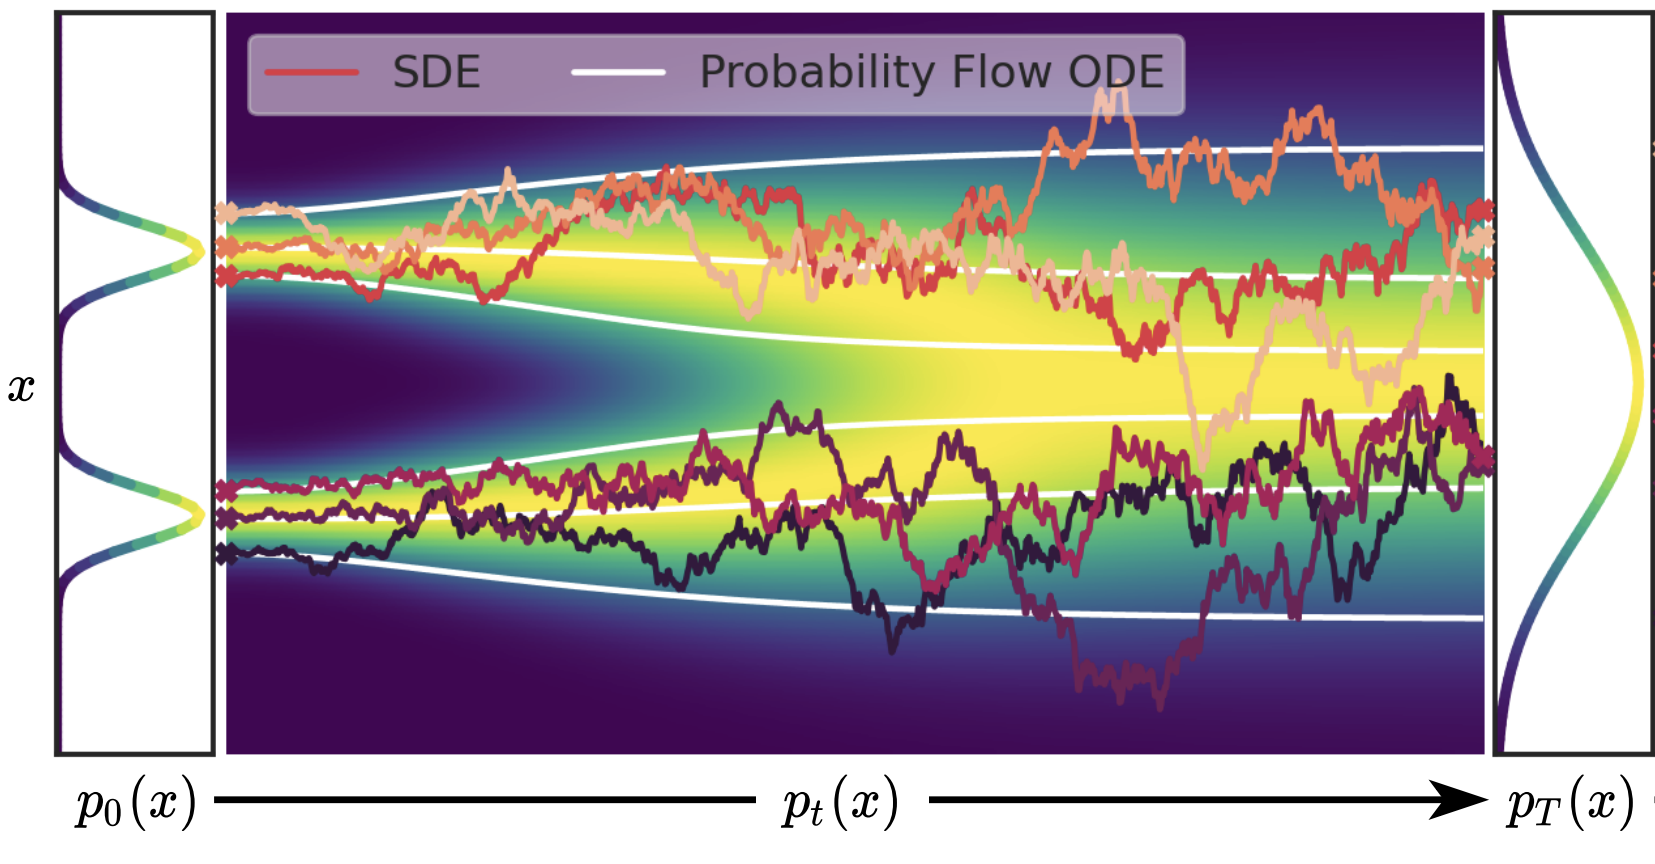
\includegraphics[width=0.75\linewidth]{figs/probability_flow}
	\end{figure}
\end{frame}
%=======
\begin{frame}{Why do we need to convert SDEs to PF-ODEs?}
	\begin{itemize}
		\item We could use \SDESolve to discretize the SDE.
		\item However, this is not efficient (trajectories are not smooth).
	\end{itemize}
	\eqpause
	\begin{block}{Efficient Solvers}
		\begin{itemize}
			\item Converting SDEs to PF-ODEs yields more efficient inference.
			\item We can apply any \ODESolve procedure to reduce the number of inference steps.
			\item For example, we can use Heun's / Runge-Kutta methods to solve the PF-ODE instead of Euler's method.
			\item In practice, this reduces the number of steps from $100$--$1000$ to $20$--$50$.
		\end{itemize}
	\end{block}
\end{frame}
%=======
\begin{frame}{Summary}
	\begin{itemize}
		\item Every SDE admits a corresponding probability flow ODE following the same probability path.
	\end{itemize}
\end{frame}
\end{document}